\chapter{Élasticité classique} \label{chap:Ch06}
\section{Équations de l'élasticité} \label{sec:Ch06-1}
\subsection{Problèmes reguliers} \label{ssec:Ch06-1.1}
Pour résoudre un problème d'élasticité, il faut trouver un champ de déplacements $u_i\left( x,t \right)$ et un champ de contraintes $\sigma_{ij}\left( x,t \right)$ vérifiant les équations du mouvement ou d'équilibre suivant que l'on s'intéresse au problème dynamique ou quasi-statique:
\begin{equation}
    \sigma_{ij,j} + f_i = \rho \frac{\partial^2 u_i}{\partial t^2} \text{ ou } 0
    \label{eq:Ch06-001}
\end{equation}
et la loi de comportement:
\begin{equation}
    \sigma_{ij} = A_{ijkl} \varepsilon_{kl}
    \label{eq:Ch06-002}
\end{equation}
où le tenseur des déformations s'écrit:
\begin{equation}
    \varepsilon_{ij} = \frac{1}{2} \left( u_{i,j} + u_{j,i} \right)
    \label{eq:Ch06-003}
\end{equation}
On obtient donc un système de neuf équations à neuf inconnues et le problème sera «~bien posé~» et admettra une solution unique pourvu qu'on lui rajoute des conditions aux limites et éventuellement des conditions initiales adéquates.
Les conditions initiales donnent la position et la vitesse du milieu à l'instant 0:
\begin{equation}
    u_i \left( x,0 \right) = u_{i}^0 (x)\quad\text{et}\quad \frac{\partial u_i}{\partial t} \left( x,0 \right) = V_i^0 \left( x \right)
    \label{eq:Ch06-004}
\end{equation}
Les différents types de conditions aux limites que l'on peut rencontrer ont été discutées au paragraphe~\ref{ssec:Ch04-1.2}.
On définit classiquement:
\begin{description}
    \item Problème de type I --- les déplacements sont donnés à la frontière:
        \begin{equation}
            u_i{}_{|_{\partial \Omega}} = u_i^d
            \label{eq:Ch06-005}
        \end{equation}
    \item Problème de type II --- les efforts appliqués au solide sur la frontière sont donnés:
        \begin{equation}
            \sigma_{ij} n_j{}_{|_{\partial \Omega}} = T_i^d
            \label{eq:Ch06-006}
        \end{equation}
\end{description}
Par exemple, le réservoir sphérique au paragraphe~\ref{ssec:Ch04-1.1} ou le bloc pesant du paragraphe~\ref{ssec:Ch04-1.2} avec la condition aux limites~\eqref{eq:Ch04-025}.

Plus généralement, on a affaire à un problème mixte pour lequel sur chaque partie de $\partial \Omega$ on donne:
\begin{itemize}
    \item les efforts, exemple~\eqref{eq:Ch04-008}; 
    \item les déplacements, exemple~\eqref{eq:Ch04-012};
    \item certaines composantes du déplacement et les composantes complémentaires de l'effort, exemple~\eqref{eq:Ch04-011}.
\end{itemize}

Un exemple type de problème mixte est celui où l'on se donne les déplacements sur une partie de la surface et les efforts sur la partie complémentaire:
\begin{equation}
    u_i{}_{|_{S_u}} =  u_i^d \quad, \quad \sigma_{ij} n_j{}_{|_{S_f}} = T_i^d
    \label{eq:Ch06-007}
\end{equation}
avec $\partial \Omega = S_u + S_f$.
C'est par exemple le cas pour les deux problèmes du paragraphe~\ref{ssec:Ch04-1.2} avec condition d'adhérence, mais pour ces mêmes problèmes avec conditions de non frottement, les conditions aux limites sur les bases donnent la composante du déplacement sur $x_3$ et les composantes de l'effort sur $x_1$, $x_2$.
De manière générale, nous introduisons la classe des problèmes réguliers, problèmes pour lesquels en tout point de la frontière $\partial \Omega$ sont données trois composantes complémentaires de l'effort $T_i = \sigma_{ij} n_j$ ou du déplacement $u_i$.
Pour qu'un problème soit régulier, il faut que l'intégrale représentant le travail des efforts de contact puisse se décomposer en deux termes:
\begin{equation}
    \iint_{\partial \Omega} \sigma_{ij} n_j u_i \ud S = T_f^d \left( u_i \right) + T_u^d \left( \sigma_{ij} \right)
    \label{eq:Ch06-008}
\end{equation}
Le premier terme $T_f^d$ représente le travail des efforts donnés dans le déplacement (inconnu) et le second, le travail des efforts de contact (inconnus) dans les déplacements donnés.
Pour le problème mixte~\eqref{eq:Ch06-007}, on a simplement\footnote{Les problèmes de type I et II sont des cas particuliers du problème mixte~\eqref{eq:Ch06-007}.}:
\begin{equation}
    \iint_{\partial \Omega} \sigma_{ij} n_j u_i \ud S = \underbrace{\iint_{S_u} \sigma_{ij} n_j u_i^d \ud S}_{T_u^d\left( \sigma_{ij} \right)} +  \underbrace{\iint_{\partial \Omega} T_i^d u_i \ud S}_{T_f^d\left( u_i \right)}
    \label{eq:Ch06-009}
\end{equation}
Pour les autres problèmes réguliers, cette décomposition est plus longue à écrire.
Par exemple, pour le problème du bloc pesant avec condition de non frottement~\eqref{eq:Ch06-019}, on a:
\begin{equation}
    \iint_{\partial \Omega} \sigma_{ij} n_j u_i \ud S = \underbrace{\iint_{S_l +S_1} T_i^d u_i \ud S - \iint_{S_0} \left( \sigma_{13}^d u_i + \sigma_{23}^d u_2 \right.}_{T_f^d\left( u_i \right)} + \underbrace{ \left.\sigma_{33} u_3^d \right)}_{T_u^d\left(\sigma_{ij} \right)} \ud S
    \label{eq:Ch06-010}
\end{equation}
Pour ce problème particulier, chacun des termes est nul d'après~\eqref{eq:Ch04-018} et~\eqref{eq:Ch04-019}, mais peu importe, l'essentiel est d'examiner ce qui est donné par les conditions aux limites et de vérifier que l'on peut effectuer la décomposition~\eqref{eq:Ch06-008} sans ambiguïté.
En particulier, il en résulte que, pour le problème homogène associé, c'est-à-dire pour le problème correspondant à toutes les données nulles, on a automatiquement:
\begin{equation}
    \iint_{\partial \Omega} \sigma_{ij} n_j u_i \ud S = 0
    \label{eq:Ch06-011}
\end{equation}
c'est un moyen commode pour vérifier qu'un problème est régulier.

Cette notion de problème régulier est essentielle car elle recouvre la formulation naturelle des conditions aux limites en Mécanique des Solides en général.
En élasticité, les problèmes réguliers sont des problèmes linéaires --~on peut donc superposer plusieurs solutions~-- et qui permettent de démontrer un certain nombre de théorèmes généraux, notamment des théorèmes d'existence et d'unicité --~un problème régulier est bien posé~-- et les théorèmes de l'énergie qui feront l'objet d'un chapitre.

Il existe des problèmes non réguliers, comme par exemple les problèmes de frottement ou les problèmes unilatéraux.
Dans les deux cas, il s'agit de conditions aux limites non linéaires qui rendent le problème non linéaire et par conséquent, beaucoup plus difficile à résoudre.
Les liaisons élastiques donnent un exemple de problème linéaire non régulier.
Nous rencontrerons aussi des problèmes non réguliers par manque de données mais il s'agit alors d'une non régularité superficielle qui ne nous gênera guère.

\subsection{Theorème d'unicité en dynamique} \label{ssec:Ch06-1.2}
Comme nous l'avons affirmé plus haut, un problème régulier est bien 
posé, autrement dit, il admet une solution unique.
\`A titre d'exemple, nous allons démontrer le théorème d'unicité dans le cas dynamique.
Nous partons donc d'un problème dynamique régulier.
Pour fixer les notations, nous prendrons des conditions aux limites mixtes de type~\eqref{eq:Ch06-007} mais la démonstration est valable, à des difficultés de notations près, pour tout problème régulier.
Nous cherchons donc $u_i\left( x,t \right)$, $\sigma_{ij}\left( x,t \right)$, $\varepsilon_{ij}\left( x,t \right)$, solutions du problème suivant:
\begin{equation}
    \left\{
    \begin{aligned}
        \rho \frac{\partial^2 u_i}{\partial t^2} &= \sigma_{ij,j} + f_i \\
        \sigma_{ij} &= A_{ijkl} \varepsilon_{kh} \\
        \varepsilon_{ij} &= \frac{1}{2} \left( u_{i,j} + u_{j,i} \right) \\
        u_i \left( x,0 \right) &= u_i^c \left( x \right) \quad & V_i\left( x,0 \right) = V_i^c\left( x \right) \\
        u_i{}_{|_{S_u}} &= u_i^d  \quad & \sigma_{ij} n_j{}_{S_f} = T_i^d
    \end{aligned}
    \right.
    \label{eq:Ch06-012}
\end{equation}
Au paragraphe~\ref{ssec:Ch01-2.1}, nous avons démontré le théorème de l'énergie cinétique~\eqref{eq:Ch01-029} mais en élasticité, il vient, d'après~\eqref{eq:Ch05-006} et~\eqref{eq:Ch05-008}:
\begin{equation}
    \sigma_{ij} D_{ij} = \sigma_{ij} \frac{\ud \varepsilon_{ij}}{\ud t} = \frac{\ud w}{\ud t}
    \label{eq:Ch06-013}
\end{equation}
ce qui permet d'écrire~\eqref{eq:Ch01-029} sous la forme:
\begin{equation}
    \frac{\ud}{\ud t} \left( K + W \right) = \iiint_{\Omega} f_i \frac{\partial u_i}{\partial t} \ud v + \iint_{\partial \Omega} \sigma_{ij} n_j \frac{\partial u_i}{\partial t} \ud S
    \label{eq:Ch06-014}
\end{equation}
où $W$ est l' énergie de déformation du so1ide:
\begin{equation}
    W = \iiint_{\Omega} w \ud v = \frac{1}{2} \iint_{\Omega} A_{ijkh} \varepsilon_{ij} \varepsilon_{kh} \ud v
    \label{eq:Ch06-015}
\end{equation}
La signification de~\eqref{eq:Ch06-014} est claire: la dérivée par rapport au temps de l'énergie totale (cinétique + de déformation) du solide est égale à la puissance des efforts extérieurs.

Supposons maintenant que notre problème~\eqref{eq:Ch06-012} admette deux solutions correspondant aux mêmes données $\left( f_i, u_i^0, V_i^0, u_i^d, T_i^d \right)$.
La différence de ces deux solutions:
\begin{equation}
    \bar{u}_i = u_i^{(2)} - u_i^{(1)}, \quad \bar{\varepsilon}_{ij} = \varepsilon_{ij}^{(2)} - \varepsilon_{ij}^{(1)}, \quad  \bar{\sigma}_{ij} = \sigma_{ij}^{(2)} - \sigma_{ij}^{(1)}
    \label{eq:Ch06-016}
\end{equation}
sera solution du problème homogène associé à~\eqref{eq:Ch06-012}:
\begin{equation}
    \bar{f}_i = 0, \quad \bar{u}_i^0 = \bar{V}_i^0 = 0, \quad \bar{T}_i^d= 0
    \label{eq:Ch06-017}
\end{equation}
En appliquant~\eqref{eq:Ch06-014} à ce problème:
\begin{equation}
    \iint_{\Omega} \bar{f}_i \frac{\partial \bar{u}_i}{\partial t} \ud v + \iint_{S_u} \bar{\sigma_{ij}} n_j \frac{\partial \bar{u}_i^d}{\partial t} \ud S + \iint_{S_f} \bar{T}_i^d \frac{\partial \bar{u}_i}{\partial t} \ud S = 0
    \label{eq:Ch06-018}
\end{equation}
est nul d'après~\eqref{eq:Ch06-017} puisque $\bar{f}_i$, $\bar{T}_i^d$ et $\bar{u}_i^d$ et donc $\partial \bar{u}_i^d/\partial t$ sont nuls.
On en déduit:
\begin{equation}
    \frac{\ud}{\ud t} \left( \bar{K} + \bar{W} \right) = 0, \quad \bar{K} + \bar{W} = \text{Cte} = 0
    \label{eq:Ch06-019}
\end{equation}
puisqu'à l'instant initial, d'après~\eqref{eq:Ch06-017}, il vient:
\begin{equation}
    \bar{u}_i \left( x,0 \right) = \frac{\partial \bar{u}_i}{\partial t} \left( x,0 \right) = 0
    \label{eq:Ch06-020}
\end{equation}
Or l'énergie cinétique $K$, par définition, et l'énergie de déformation $W$ d'après le postulat de stabilité~\eqref{eq:Ch04-004}, sont définies positives, d'où il résulte que $\bar{K}$ et $\bar{W}$ restent nuls au cours du temps.
On a donc en tout point et à tout instant $\partial \bar{u}_i/\partial t = 0$ d'où:
\begin{equation}
    \bar{u}_i \left( x,t \right) = 0, \quad u_i^{(2)} \left( x,t \right) = u_i^{(1)} \left( x,t \right)
    \label{eq:Ch06-021}
\end{equation}
Les deux solutions coïncident et le problème~\eqref{eq:Ch06-012} a une solution unique.
Nous démontrerons au chapitre \ref{chap:Ch09} le théorème d'unicité peur le problème statique, mais provisoirement nous l'admettrons.

\subsection{Équations de Navier} \label{ssec:Ch06-1.3}
Pour résoudre analytiquement un problème d'élasticité, on postule \textit{a priori} une forme particulière pour la solution puis on essaie de vérifier toutes les équations.
Si on y parvient, alors d'après le théorème d'unicité pour un problème régulier, c'est la solution du problème.
Il en résulte donc deux méthodes, suivant que l'on essaie un champ de déplacement ou un champ de contraintes.

Si l'on part du champ de déplacement $u_i$ on peut calculer le tenseur des déformations par~\eqref{eq:Ch06-003} et le tenseur des contraintes par la loi de comportement~\eqref{eq:Ch06-002}.
Il ne reste donc plus à vérifier que les équations du mouvement~\eqref{eq:Ch06-001}, les conditions aux limites de type déplacement et de type effort et éventuellement les conditions initiales.
Reporter~\eqref{eq:Ch06-002} et~\eqref{eq:Ch06-003} dans l'équation du mouvement~\eqref{eq:Ch06-001} permet d'écrire l'équation qui doit être vérifiée par le champ de déplacements $u_i\left( x,t \right)$ en dynamique ou $u_i(x)$ en statique:
\begin{equation}
    A_{ijkh} \frac{\partial^2 u_k}{\partial x_j \partial x_h} + f_i = \rho \frac{\partial^2 u_i}{\partial t^2} \text{ ou } 0
    \label{eq:Ch06-022}
\end{equation}
où la symétrie~\eqref{eq:Ch05-003} de $A_{ijkh}$ est utilisée et en supposant le matériau homogène ($A$ constant).
En élasticité, le temps n'intervient pas dans la loi de comportement.
Il n'intervient que dans l'équation du mouvement et disparaît en quasi-statique à l'exception des problèmes de frottement, où il reste dans la condition aux limites~\eqref{eq:Ch04-015}.
Ainsi en élasticité, on ne parle jamais de problèmes quasi-statiques mais uniquement de problèmes statiques.
Pour résoudre un problème quasi-statique, il suffit en effet de résoudre à chaque instant le problème statique correspondant.
Nous n'envisagerons plus désormais que le cas statique.

Dans le cadre de l'élastictté linéaire isotrope ---élasticité classique--- l'équation~\eqref{eq:Ch06-022} devient d'après~\eqref{eq:Ch05-023}:
\begin{equation}
    \left( \lambda + \mu \right) u_{i,ik} + \mu u_{i,kh} + f_i = 0
    \label{eq:Ch06-023}
\end{equation}
soit, en introduisant les opérateurs de l'analyse vectorielle (Annexe~\ref{Ann:A}):
\begin{equation}
    \left( \lambda + \mu \right) \grad \left( \dive \vec{u} \right) + \mu \Delta \vec{u} + \vec{f} = 0
    \label{eq:Ch06-024}
\end{equation}
ou de manière équivalente:
\begin{equation}
    \left( \lambda + 2\mu \right) \grad \dive \vec{u} - \mu \rot \rot \vec{u} + \vec{f} = 0
    \label{eq:Ch06-025}
\end{equation}
Ces équations sont appelées les équations de Navier.
Elles traduisent les équations d'équilibre pour le champ des déplacements.

Ainsi la première méthode de résolution d'un problème d'élastostatique consiste à: 
\begin{itemize}
    \item postuler un champ de déplacements;
    \item vérifier les équations de Navier~\eqref{eq:Ch06-024} ou~\eqref{eq:Ch06-025};
    \item vérifie, les conditions aux limites de type déplacement;
    \item vérifier les conditions aux limites de type effort.
\end{itemize}
Pour postuler le champ de déplacements, on s'inspire habituellement des conditions aux limites en déplacement et des symétries.
On verra des exemples de cette méthode aux paragraphes~\ref{ssec:Ch06-2.2} et~\ref{ssec:Ch07-2.1}. 

Si on prend la divergence de l'équation~\eqref{eq:Ch06-025}, on obtient l'équation de la dilatation
\begin{equation}
    \left( \lambda + 2 \mu \right) \Delta \left( \dive \vec{u} \right) + \dive \vec{f} = 0
    \label{eq:Ch06-026}
\end{equation}
qui nous sera utile plus loin.

\subsection{Équations de Beltrami} \label{ssec:Ch06-1.4}
La seconde méthode de résolution consiste à postuler un champ de contraintes.
La loi de comportement permet alors de calculer le champ des déformations, mais pour pouvoir calculer le vecteur déplacement, il faut que ce champ de déformations soit compatible (paragraphe~\ref{sec:Ch03-3}).
Ainsi, le champ de contraintes choisi doit vérifier les équations d'équilibre et un système d'équations traduisant les équations de compatibilité.
Nous allons obtenir ce système d'équations dans le cas statique et en élasticité classique et homogène.

Nous partons des équations de compatibilité sous la forme~\eqref{eq:Ch03-060} et de la loi de comportement sous la forme~\eqref{eq:Ch05-034}, ainsi:
\begin{equation*}
    \left( \frac{1+\nu}{E} \sigma_{ij} - \frac{\nu}{E} \sigma_{kk} \delta_{ij} \right)_{,ll} + \frac{1 - 2\nu}{E} \sigma_{kk,ij} - \frac{1+ \nu}{E} \left( \sigma_{jk,ik} + \sigma_{ik,jk} \right) + \frac{2\nu}{E} \sigma_{kk,ij} = 0
\end{equation*}
et en notation indicielle:
\begin{equation}
    \left( 1+\nu \right)\sigma_{ij,ll} - \nu \sigma_{kk,ll} \delta_{ij} + \sigma_{kk,ij} - \left( 1+\nu \right) \left[ \sigma_{jk,ki} + \sigma_{ik,kj} \right] = 0
    \label{eq:Ch06-027}
\end{equation}
mais d'après les équations d'équilibre~\eqref{eq:Ch06-001}:
\begin{equation}
    \sigma_{jk,ki} + \sigma_{ik,kj} = - \left( f_{i,j} + f_{j,i} \right)
    \label{eq:Ch06-028}
\end{equation}
et d'après la loi de comportement~\eqref{eq:Ch05-034} et l'équation de la dilatation~\eqref{eq:Ch06-026}:
\begin{equation*}
    \sigma_{kk,ll} = \frac{E}{1-2\nu} \varepsilon_{kk,ll} = - \frac{E}{\left( \lambda + 2\mu \right)\left( 1-2\nu \right)}f_{i,i}
\end{equation*}
soit finalement avec~\eqref{eq:Ch05-033}:
\begin{equation}
    \sigma_{kk,ll} = - \frac{1+\nu}{1-\nu} f_{i,i}
    \label{eq:Ch06-029}
\end{equation}
En eeportant~\eqref{eq:Ch06-028} et~\eqref{eq:Ch06-029} dans~\eqref{eq:Ch06-027}, on obtient:
\begin{equation}
    \sigma_{ij,ll} + \frac{1}{1+\nu} \sigma_{kk,ij} + f_{i,j} + f_{j,i} + \frac{\nu}{1-\nu} f_{i,i} = 0
    \label{eq:Ch06-030}
\end{equation}
Ces équations, appelées équations de Beltrami, traduisent les équations de compatibilité pour les contraintes.
Si les forces de volume sont nulles, elles se simplifient:
\begin{equation}
    \sigma_{ij,ll} + \frac{1}{1+\nu} \sigma_{kk,ij} = 0
    \label{eq:Ch06-031}
\end{equation}
En particulier, elles seront automatiquement vérifiées si les contraintes sont des fonctions linéaires des coordonnées.

La seconde méthode de résolution d'un problème élasto-statique consiste à: 
\begin{itemize}
    \item postuler un champ de contraintes;
    \item vérifier les équations d'équilibre;
    \item vérifier les équations de Beltrami;
    \item vérifier les conditions aux limites de type effort;
puis, le cas échéant 
\end{itemize}
\begin{itemize}
    \item intégrer le champ de déplacements;
    \item  vérifier les conditions aux limites de type déplacement.
\end{itemize}
On voit donc que cette méthode s'applique tout naturellement aux problèmes de type II pour lesquels on peut sauter les deux dernières étapes.
Nous en verrons des exemples aux paragraphes~\ref{ssec:Ch06-2.1}, \ref{ssec:Ch07-2.2} et~\ref{ssec:Ch07-3.1}.

\section{Problèmes simples} \label{sec:Ch06-2}
Comme premier exemple, on peut citer le problème de la compression d'un lopin avec conditions aux limites de non frottement qui a été résolu de manière tout à fait générale au paragraphe~\ref{ssec:Ch04-1.3}.
Nous allons traiter deux autres exemples issus du paragraphe~\ref{sec:Ch04-1}.
\subsection{Déformation d'un bloc pesant} \label{ssec:Ch06-2.1}
Nous considérons donc le problème du bloc pesant posé sur un ballon de baudruche (paragraphe~\ref{ssec:Ch04-1.3}).
On aura donc $f_i = -\rho g$ et les conditions aux limites sont:
\begin{equation}
    \left\{
    \begin{aligned}
        & \sigma_{ij} n_j = 0 \text{ sur } S_2 \\
        & x_3 = h:\ \sigma_{13} = \sigma_{23} = \sigma_{33} = 0 \\
        & x_3 = 0:\ \sigma_{13} = \sigma_{23} = 0, \ \sigma_{33} = -p
    \end{aligned}
    \right.
    \label{eq:Ch06-032}
\end{equation}

\begin{center}
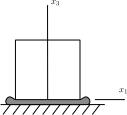
\includegraphics{../images/T1_Ch06-01}
\end{center}  

C'est un problème régulier de type II et par conséquent, la solution sera donc unique: ceci conduit à rechercher le champ de contraintes.
Les trois équations d'équilibre s'écrivent:
\begin{equation}
    \left\{
    \begin{aligned}
        \sigma_{11,1} + \sigma_{12,2} + \sigma_{13,3} &= 0 \\
        \sigma_{12,1} + \sigma_{22,2} + \sigma_{23,3} &= 0 \\
        \sigma_{13,1} + \sigma_{23,2} + \sigma_{33,3} &= \rho g
    \end{aligned}
    \right.
    \label{eq:Ch06-033}
\end{equation}
Les conditions aux limites sur la surface latérale s'écrivent, avec $\vec{n} = \left( n_1, n_2, 0 \right)$:
\begin{equation}
    \left\{
    \begin{aligned}
        \sigma_{11}n_1 + \sigma_{12}n_2 &= 0 \\
        \sigma_{21}n_1 + \sigma_{22}n_2 &= 0 \\
        \sigma_{31}n_1 + \sigma_{32}n_2 &= 0
    \end{aligned}
    \right.
    \label{eq:Ch06-034}
\end{equation}
L'examen de ces équations nous conduit à chercher le tenseur des contraintes sous la forme:
\begin{equation}
    \tens{\sigma} = 
    \begin{bmatrix}
        0 & 0 & 0 \\
        0 & 0 & 0 \\
        0 & 0 & \sigma_{33}(x)
    \end{bmatrix}
    \label{eq:Ch06-035}
\end{equation}
qui vérifie automatiquement:
\begin{itemize}
    \item les conditions aux 1imites~\eqref{eq:Ch06-034} sur $S_l$;
    \item les conditions aux aimites portant sur $\sigma_{13}$ et $\sigma_{23}$ en $x_3 = 0$ et $x_3 =h$.
\end{itemize}
Les équations d'équilibre donnent alors:
\begin{equation*}
    \sigma_{33} = \rho g x_3 = \text{Cte}
\end{equation*}
et les conditions aux limites en $x_3=h$ et $x_3=0$ entraînent:
\begin{equation}
    \sigma_{33} = \rho g \left( x_3 -h \right), \quad p = \rho g h
    \label{eq:Ch06-036}
\end{equation}
On retrouve donc~\eqref{eq:Ch04-027}.
Par ailleurs, ce champ de contraintes est linéaire et vérifie automatiquement les équations de Beltrami~\eqref{eq:Ch06-031} ($f_i = \text{Cte}$).
Ainsi, le champ de contraintes~\eqref{eq:Ch06-035} et~\eqref{eq:Ch06-036} vérifie toutes les équations du problème.
C'est la solution.

Si l'on veut connaître le déplacement, il faut faire appel à la loi de comportement:
\begin{equation}
    \tens{\varepsilon} = \frac{1}{E} 
    \begin{bmatrix}
        -\nu \rho g x_3' & 0 & 0 \\
        0 & -\nu \rho g x_3' & 0 \\
        0 & 0 & \rho g x_3'
    \end{bmatrix}
    \label{eq:Ch06-037}
\end{equation}
en prenant $x_3'= x_3 -h$, c'est-à-dire en prenant l'origine des coordonnées sur la face supérieure du bloc.
Par rapport à cette nouvelle variable, le champ des déformations est linéaire et on peut appliquer la formule~\eqref{eq:Ch03-065} pour le calcul du déplacement. On peut aussi procéder directement à partir de~\eqref{eq:Ch06-003}.
En effet:
\begin{equation}
    \left\{
    \begin{aligned}
        & \varepsilon_{33} = \frac{\partial u_3}{\partial x_3'} = \frac{1}{E} \rho g x_3' &\Rightarrow E u_3 = \frac{1}{2}\rho g x_3'^2 + \varphi_3 \left( x_1, x_2 \right) \\
        & \varepsilon_{11} = \frac{\partial u_1}{\partial x_1} = \frac{-\nu}{E} \rho g x_3' &\Rightarrow E u_1 = -\nu\rho g x_3'^2 + \varphi_1 \left( x_2, x_3 \right) \\
        & \varepsilon_{22} = \frac{\partial u_2}{\partial x_2} = \frac{-\nu}{E} \rho g x_3' &\Rightarrow E u_2 = -\nu\rho g x_3'^2 + \varphi_2 \left( x_3, x_1 \right)
    \end{aligned}
    \right.
    \label{eq:Ch06-038}
\end{equation}
\begin{equation}
    \left\{
    \begin{aligned}
        & 2\varepsilon_{12} = \frac{\partial u_1}{\partial x_2} + \frac{\partial u_2}{\partial x_1} = \varphi_{1,2} + \varphi_{2,1} = 0 \\
        & 2\varepsilon_{13} = \frac{\partial u_1}{\partial x_3'} + \frac{\partial u_3}{\partial x_1} = -\nu \rho g x_1 + \varphi_{1,3} + \varphi_{3,1} = 0 \\
        & 2\varepsilon_{23} = \frac{\partial u_2}{\partial x_3'} + \frac{\partial u_3}{\partial x_2} = -\nu \rho g x_2 + \varphi_{2,3} + \varphi_{3,2} = 0 \\
    \end{aligned}
    \right.
    \label{eq:Ch06-039}
\end{equation}
et on obtient une solution particulière:
\begin{equation}
    \varphi_1 = \varphi_2 = 0 ,\quad \varphi_3 = + \frac{1}{2}\nu\rho g \left( x_1^2 + x_2^2 \right)
    \label{eq:Ch06-040}
\end{equation}
d'où finalement la solution, en revenant à $x_3$:
\begin{equation}
    \left\{
    \begin{aligned}
        E u_1 & = -\nu \rho g x_1 \left( x_3 - h \right) \\
        E u_2 & = -\nu \rho g x_2 \left( x_3 - h \right) \\
        E u_3 & = \frac{1}{2} \rho g \bigl[ \left( x_3 - h \right)^2 + \nu \left( x_1^2 + x_2^2 \right)  \bigr]
    \end{aligned}
    \right.
    \label{eq:Ch06-041}
\end{equation}
à un déplacement de solide près.
\begin{multicols}{2}
    \begin{center}
        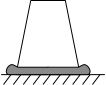
\includegraphics{../images/T1_Ch06-02}
    \end{center}
    \columnbreak
    On en déduit l'allure de la déformation du bloc.
\end{multicols}
\subsection{Réservoir sphérique sous pression} \label{ssec:Ch06-2.2}
\begin{multicols}{2}
    Nous considérons le réservoir sphérique sous pression du paragraphe~\ref{sec:Ch04-1} avec $f_i = 0$ et les conditions aux limites suivantes:
    \begin{equation}
        \left\{
        \begin{aligned}
            r=a &:& \sigma_{ij} n_j = -p n_i \\
            r=b &:& \sigma_{ij} n_j = 0
        \end{aligned}
        \right.
        \label{eq:Ch06-042}
    \end{equation}
    \columnbreak
    \begin{center}
        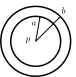
\includegraphics{../images/T1_Ch06-03}
    \end{center}
\end{multicols}
Compte-tenu de la symétrie du problème, on peut supposer que le vecteur déplacement est radial et ne dépend que de la distance au centre $r=OM$:
\begin{equation}
    u_i = g(r) x_i,\quad
    r^2 = x_i x_i;\quad \frac{\partial r}{\partial x_i} = r_{,i} = \frac{x_i}{r}
    \label{eq:Ch04-044}
\end{equation}
Un calcul direct donne alors:
\begin{equation}
    u_{i,j} = g(r) \delta_{ij} + \frac{g'(r)}{r} x_i x_j = \varepsilon_{ij}
    \label{eq:Ch06-045}
\end{equation}
Le gradient du déplacement étant symétrique, il s'ensuit que son rotationnel $\rot \vec{u}$ est nul.
L'équation de Navier~\eqref{eq:Ch06-025} donne alors:
\begin{equation}
    \grad \left( \dive \vec{u} \right) = 0 ,\quad \dive \vec{u} = \text{Cte} = 3 \alpha
    \label{eq:Ch06-046}
\end{equation}
Compte-tenu de~\eqref{eq:Ch06-045}, il vient:
\begin{equation}
    u_{i,j} = 3 g(r) + \frac{g'(r)}{r} = 3 \alpha
    \label{eq:Ch06-047}
\end{equation}
et par intégration:
\begin{equation}
    g(r) = \alpha + \frac{\beta}{r^3}
    \label{eq:Ch06-048}
\end{equation}
Il reste à déterminer les constantes d'intégration $\alpha$ et $\beta$ pour vérifier les conditions aux limites~\eqref{eq:Ch06-042}.
Pour cela, nous devons calculer les contraintes:
\begin{equation}
    \varepsilon_{ij} = \left( \alpha + \frac{\beta}{r^3} \right)\delta_{ij} - \frac{3\beta x_i x_j}{r^5}
    \label{eq:Ch06-049}
\end{equation}
et nous allons écrire la loi de comportement sous la forme~\eqref{eq:Ch06-039}.
En effet, la décomposition de~\eqref{eq:Ch06-049} en partie sphérique et déviateur donne directement:
\begin{equation}
    \begin{aligned}
        &\varepsilon = \frac{1}{3} \varepsilon_{ii} = \alpha && \Rightarrow && \sigma = 3K  \alpha \\
        &e_{ij} = \frac{\beta}{r^3} \left( \delta_{ij} - 3 \frac{x_ix_j}{r^2} \right) && \Rightarrow && s_{ij} = \frac{2\mu\beta}{r^3} \left( \varepsilon_{ij} - 3 \frac{x_i x_j}{r^2} \right)
    \end{aligned}
    \label{eq:Ch06-050}
\end{equation}
D'où finalement:
\begin{equation}
    \sigma_{ij} = \left( 3K\alpha + 2\mu \frac{\beta}{r^3} \right) \delta_{ij} - \frac{6\mu\beta}{r^3} \frac{x_ix_j}{r^2}
    \label{eq:Ch06-051}
\end{equation}
Le tenseur des contraintes est de révolution autour de la direction radiale et les contraintes principales sont:
\begin{equation}
    \sigma_1 = \sigma_2 = 3 K \alpha + \frac{2\mu\beta}{r^3}, \quad \sigma_3 = 3 K \alpha - \frac{4\mu\beta}{r^3}
    \label{eq:Ch06-052}
\end{equation}
avec $\sigma_3$ associé à la direction radiale.
La condition~\eqref{eq:Ch06-042} s' écrit alors simplement puisque sur les deux sphères frontières, la normale est radiale:
\begin{equation}
    \left\{
    \begin{aligned}
        r=a & : && \sigma_3 = 3K\alpha - \frac{4\mu\beta}{a^3} = -p \\
        r=b & : && \sigma_3 = 3K\alpha - \frac{4\mu\beta}{b^3} = 0
    \end{aligned}
    \right.
    \label{eq:Ch06-053}
\end{equation}
On obtient ainsi un système de deux équations à deux inconnues qui donne les constantes d'intégration $\alpha$ et $\beta$ par:
\begin{equation}
    4\mu\beta = \frac{pa^3b^3}{b^3-a^3}; \quad 3K\alpha = \frac{p a^3}{b^3-a^3}
    \label{eq:Ch06-054}
\end{equation}
et la solution est complètement déterminée.

Il reste à écrire la condition de limite élastique.
Si l'on adopte le critère de von Mises, alors il vient directement, par exemple à partir de~\eqref{eq:Ch06-050} et~\eqref{eq:Ch05-065}:
\begin{equation}
    \frac{1}{2} s_{ij} s_{ij} = \frac{12 \mu^2 \beta^2}{r^4} \leq \frac{\sigma_e^2}{3}
    \label{eq:Ch06-055}
\end{equation}
Si l'on adopte le critère de Tresca, alors à partir de~\eqref{eq:Ch06-052} et~\eqref{eq:Ch05-070}:
\begin{equation}
    \sigma_1 - \sigma_3 = \frac{6\mu\beta}{r^3} \leq \sigma_e
    \label{eq:Ch06-056}
\end{equation}
Les deux critères donnent donc le même résultat, ce qui était évident \textit{a priori} puisque l'état de contraintes est de révolution, c'est donc, à un tenseur sphérique près, un état de traction simple pour lequel Tresca et von Mises coincident par construction.
Ainsi le calcul élastique est justifié si la condition:
\begin{equation}
    \frac{3pa^3b^3}{2\left( b^3 -a^3 \right)r^3} \leq \sigma_e
    \label{eq:Ch06-057}
\end{equation}
est vérifiée en tout point.
Le point le plus sollicité sera donc le point où $r$ est minimum, c'est-à-dire à l'intérieur ($r=a$).
On obtient donc la condition:
\begin{equation}
    \frac{3}{2}\frac{pb^3}{b^3-a^3} \leq \sigma_e ; \quad p \leq p_e = \frac{2\sigma_e}{3} \left( 1 - \frac{a^3}{b^3} \right)
    \label{eq:Ch06-058}
\end{equation}
qui donne la pression maximale que peut supporter le réservoir en restant dans le domaine élastique.
En particulier, quelles que soient les dimensions du réservoir, on ne peut pas dépasser la pression limite $2\sigma_e/3$.
Nous reviendrons sur ce problème en plasticité au chapitre~\ref{chap:Ch10}.

La solution générale~\eqref{eq:Ch06-051} que nous avons obtenue permet de traiter également d'autres problèmes:
\begin{itemize}
    \item réservoir sphérique soumis à une pression intérieure $p$ et une pression extérieure $P$.
        On obtient alors:
        \begin{equation}
            3K\alpha = \frac{p a^3 - P b^3}{b^3 - a^3} ;\quad 4\mu\beta = \frac{p-P}{b^3-a^3}a^3 b^3
            \label{eq:Ch06-059}
        \end{equation}
    \item cavité sphérique dans un milieu infini:
        \begin{equation}
            4\mu\beta = p a^3; \quad 3 K \alpha = 0
            \label{eq:Ch06-060}
        \end{equation}
    \item boule dans un fluide à la pression $P$:
        \begin{equation}
            3K\alpha = -P;\quad 4 \mu\beta = 0
            \label{eq:Ch06-061}
        \end{equation}
\end{itemize}
mais, pour ce dernier problème, il est inutile d'aller chercher si loin.
Soit, en effet, un solide $\Omega$ immergé dans un fluide à la pression $P$.
En négligeant les forces de volume, on doit résoudre le problème de type II défini par les conditions aux limites:
\begin{equation}
    \sigma_{ij} n_j = -P n_i \quad \text{sur} \quad \partial \Omega
    \label{eq:Ch06-062}
\end{equation}
La solution de ce problème est triviale, quelle que soit la forme du solide:
\begin{equation}
    \sigma_{ij} = -P \delta_{ij}; \quad u_i = -\frac{P}{3K} x_i
    \label{eq:Ch06-063}
\end{equation}
On pourrait faire une étude analogue à celle du paragraphe~\ref{ssec:Ch04-1.3} et montrer que cette solution peut s'étendre à toute loi de comportement.
